\subsection{Complejidad de los algoritmos}\label{subsection:Complejidad_de_los_algoritmos}
Según \cite{[Lleida]} un algoritmo es un procedimiento o método de cálculo (con reglas bien determinadas) que conduce a la resolución de cualquier `instancia' de un problema específico (en un número finito de pasos), la complejidad o costo de un algoritmo es una medida de los recursos (tiempo, memoria) que requiere su ejecución en función del tamaño de los datos de entrada (independiente de la arquitectura de la computadora).\\
\hspace*{1cm}Una vez desarrollado un algoritmo que funciona correctamente, es necesario  definir criterios para medir su rendimiento o comportamiento. Estos criterios se centran principalmente en su simplicidad y en el uso eficiente de los recursos.\\ 
\hspace*{1cm}Según \cite{[GUE99]}, respecto al uso eficiente de los recursos, éste suele medirse en función de dos parámetros: el espacio, es decir, la memoria que utiliza, y el tiempo, lo que tarda en ejecutarse. Ambos representan los costos que supone encontrar la solución al problema planteado mediante un algoritmo. Dichos parámetros van a servir además para comparar algoritmos entre sí, permitiendo determinar el más adecuado de entre varios que solucionan un mismo problema.\\
\hspace*{1cm}El tiempo de ejecución de un algoritmo va a depender de diversos factores como son los datos de entrada que se le suministre, la calidad del código generado por el compilador para crear el programa objeto, la naturaleza y rapidez de las instrucciones máquina del procesador concreto que ejecute el programa y la complejidad intrínseca del algoritmo. Hay dos estudios posibles sobre el tiempo:

\begin{itemize}
\item Uno que proporciona una medida teórica (a priori), que consiste en obtener una función que acote el tiempo de ejecución del algoritmo para unos valores de entrada dados.
\item Otro que ofrece una medida real (a posteriori), consistente en medir el tiempo de ejecución del algoritmo para unos valores de entrada dados y una computadora específica.
\end{itemize}

\hspace*{1cm}Ambas medidas son importantes puesto que si bien la primera  ofrece estimaciones del comportamiento de los algoritmos de forma independiente de  la computadora en donde serán implementados y sin necesidad de ejecutarlos, la segunda representa las medidas reales del comportamiento del algoritmo. Estas medidas son funciones temporales de los datos de entrada.\\
\hspace*{1cm}Se entiende por tamaño de la entrada el número de componentes sobre los que se va a ejecutar el algoritmo. Por ejemplo, la dimensión del vector a ordenar o el tamaño de las matrices a multiplicar.\\ 
\hspace*{1cm}Teóricamente el tiempo de ejecución debe indicar el número de instrucciones ejecutadas por una computadora imaginaria, por tanto se deben buscar medidas simples y abstractas, independientes de la computadora a utilizar.\\
\hspace*{1cm}La unidad de tiempo a la que deben hacer referencia estas medidas de eficiencia no puede ser expresada en segundos o en otra unidad de tiempo concreta, pues no existe una computadora estándar al que puedan hacer referencia todas las medidas. Se entenderá como tiempo de ejecución a la cantidad de instrucciones en relación al número de entradas que reciba.\\
\hspace*{1cm} Como se puede observar en la figura \ref {fig:Cap2_1_1} hay 3 fórmulas donde el eje horizontal sería la cantidad de parámetros a introducir y el eje vertical es el tiempo de ejecución.

    \begin{figure}[hbtp]
        \centering
            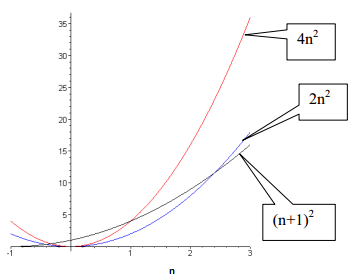
\includegraphics{MarcoTeorico/Imagenes/Cap2_1_1.png}
            \caption{Complejidad de los algoritmos.}      
            \label{fig:Cap2_1_1}
    \end{figure}    
    
    
\subsubsection{Orden de los algoritmos}
Por lo general la mayoría de los problemas tienen un parámetro de entrada que es el número de datos que hay que tratar, esto es, N. La cantidad de recursos del algoritmo es tratada como una función de N. 
Según \cite {[NIVIZI]} de esa manera puede establecerse un tiempo de ejecución del algoritmo que suele ser proporcional a una de las siguientes funciones:
\begin{itemize}
\item \textbf{$1$ (Tiempo de ejecución constante): }Significa que la mayoría de las instrucciones se ejecutan una cantidad  constante de tiempo.
\item \textbf{$logN$ (Tiempo de ejecución logarítmico): }Se puede considerar como una gran constante. La base del logaritmo (la más común es 2) cambia la constante, pero no demasiado. El programa es más lento cuanto más crezca \textit{N}, pero es inapreciable, pues \textit{logN} no se duplica hasta que \textit{N} llegue a $N^2$.
\item \textbf{$N$ (Tiempo de ejecución lineal): }Estos algoritmos puede resumirse como un bucle que se repite un número \textit{N} fijo de veces. Un caso en el que \textit{N} valga 40, tardará el doble que otro en que \textit{N} valga 20, pero si \textit{N} vale 30 tendría un tiempo intermedio de los \textit{N} anteriores. 
\item \textbf{$NlogN$ (Tiempo de ejecución en $NlogN$ ): }Es común encontrarlo en algoritmos como Quick Sort y otros del estilo divide y vencerás. Si N se duplica, el tiempo de ejecución es ligeramente mayor del doble.
\item \textbf{$N^2$ (Tiempo de ejecución cuadrático): }Suele ser habitual cuando se tratan pares de elementos de datos, como por ejemplo un bucle anidado doble. Si \textit{N} se duplica, el tiempo de ejecución aumenta cuatro veces. El peor caso de entrada del algoritmo Quick Sort se ejecuta en este tiempo.
\item \textbf{$N^3$ (Tiempo de ejecución cúbico): }Como ejemplo se puede dar el de un bucle anidado triple. Si \textit{N} se duplica, el tiempo de ejecución se multiplica por ocho.
\item \textbf{$2^N$ (Tiempo de ejecución exponencial): }No suelen ser muy útiles en la práctica por el elevado tiempo de ejecución. El problema de la mochila resuelto por un algoritmo de búsqueda exhaustiva es un ejemplo. Si N se duplica, el tiempo de ejecución crece de manera exponencial (de ahí el nombre).
\item \textbf{$n!$ (Tiempo de ejecución factorial): }La mayoría de ellos son intratables debido a que su exponente es igual al número de entradas que recibe. Si se aplica búsqueda exhaustiva a TSP, el tiempo de ejecución sería factorial.
\end{itemize}

En la figura \ref {fig:Ordenes_de_complejidad} se presenta una gráfica con el orden de crecimiento de cada uno de los conceptos en relación a su número de entradas y el tiempo que se tarda en resolverla.\\
\begin{figure}[hbtp]
    \centering
        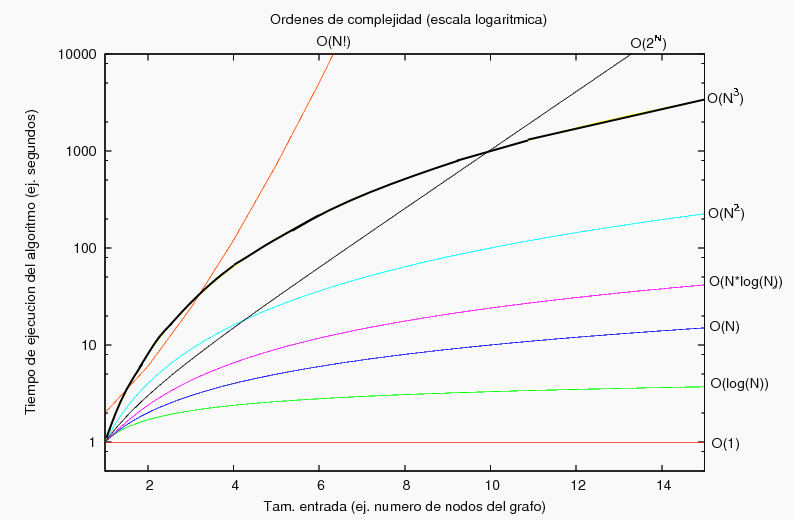
\includegraphics[width=0.8\textwidth]{MarcoTeorico/Imagenes/Ordenes_de_complejidad.png}
        \caption{Ordenes de complejidad.}      
        \label{fig:Ordenes_de_complejidad}
\end{figure}   

\subsubsection{Clasificación de los problemas}
Los problemas que tratan de resolver con algoritmos se pueden clasificar de diferentes perspectivas. De acuerdo con \cite{[MIGADA]} se tienen estas posibles clasificaciones:
\begin{enumerate}
\item 
\textbf{Por su naturaleza: }Se toma en cuenta la dificultad para resolver los algoritmos.
    \begin{itemize}
    \item \textbf{No computables: }Problemas que no admiten solución algorítmica, los problemas no computables que se basan en decisiones se llaman indecidibles.
    \item \textbf{Tratables:}Son los problemas para los cuales existen algoritmos de complejidad polinomial para resolverlos.
    \item \textbf{No tratables: }Son problemas que admiten solución y para los cuales de manera comprobada no pueden ser resueltos por algoritmos de complejidad polinomial.
    \end{itemize}
\item 
\textbf{Por el tipo de respuesta: }Es el determinar o responder SI o NO a una pregunta dada o solicitada.
\begin{itemize}
    \item \textbf{Problemas de decisión: }Es el determinar o responder SI o NO a una pregunta dada o solicitada.
    \item \textbf{Problemas de búsqueda: }Tienen como objetivo encontrar, en caso que exista, una estructura que verifique las restricciones del problema, dicha estructura es denominada de solución viable.
    \item \textbf{Problemas de optimización: }Comparte el mismo objetivo que los problemas de búsqueda pero este tipo en particular tiene que encontrar una estructura que optimice un criterio pre-definido es decir, debe encontrar la mejor solución. 
\end{itemize}
\item 
\textbf{Por su Tratabilidad: }Los problemas que admiten solución son clasificados de acuerdo a la complejidad que presentan los algoritmos para resolverlos.
\begin{itemize}
\item \textbf{La clase P: }Está constituida por todos los problemas que pueden ser resueltos por algoritmos de complejidad polinomial en una máquina convencional (máquina de Turing deterministica).
\item \textbf{La clase NP: }Es el conjunto de problemas que pueden ser resueltos en tiempo polinómico por una máquina de Turing no determinista, también contiene todos los problemas pertenecientes a las clases P, estos problemas tienen algoritmos ineficientes
\item \textbf{La clase NP-Completo: } Se dice que un problema es NP-completo si todos los problemas de la clase NP pueden reducirse a él, son los problemas más difíciles de la clase de problemas NP. Debido a la reducción, si se encuentra un algoritmo en tiempo polinomial para un problema NP-completo, se sabría que todos los problemas de la clase NP requieren un tiempo polinómico para resolverse.

\end{itemize}
\end{enumerate}

\subsubsection{Ejemplos de problemas NP-Completos}
Existen varios problemas NP-Completos, entre los más representativos se encuentran el problema de satisfacibilidad booleana y el problema del agente viajero 

\hspace*{1cm}\textbf{El problema de satisfacibilidad booleana:} De acuerdo a \cite{[Wilf]} el problema de satisfacibilidad booleana (SAT) fue el primer problema identificado como perteneciente a la clase de complejidad NP-completo en 1971. Según \cite{[Wilf]} el objetivo de SAT se enfoca a encontrar una asignación de valores a un conjunto de variables lógicas que son utilizadas para construir una fórmula lógica, de forma que dicha asignación produzca que ésta sea verdadera (una asignación satisfacible).\\
\hspace*{1cm}Normalmente la fórmula lógica se debe presentar en su forma normal conjuntiva (FNC) donde las variables lógicas se agrupan en claúsulas, que son una conjunción de literales. Como ejemplo considerando el siguiente conjunto de variables $x_1, x_2, x_3, x_4$ se tiene una fórmula lógica en su forma normal conjuntiva (FNC).
  $$(x_1 \lor \neg x_3 \lor x_4) \land (\neg x_2 \lor x_3 \lor \neg x_4)$$
\hspace*{1cm}Como se muestra en la tabla \ref{table:Cap2_1}  se verifican todas las combinaciones posibles de entradas en la que 10 de las 16 posibles generan una asignación verdadera lo que lo convierte en satisfacible. Por el contrario, si no existiera ninguna asignación que generara un resultado verdadero, entonces la fórmula sería insatisfacible.\\  

 \begin{table}[hbtp]
 \centering
    \caption{Ejemplo de satisfacibilidad booleana.} 
    \begin{tabular}{ | l | l | l | l | c |  }
    \hline
      \rowcolor[gray]{0.5}
       $x_1$ & $x_2$ & $x_3$ & $x_4$ & $(x_1\lor\neg x_3\lor x_4)\land(\neg x_2\lor x_3\lor\neg x_4) $ \\ \hline 
         V & V & V & V & V \\ \hline
         F & V & V & V & V \\ \hline
         V & F & V & V & V \\ \hline
         V & V & F & V & F \\ \hline
         V & V & V & F & V \\ \hline
         F & F & V & V & V \\ \hline
         F & V & F & V & F \\ \hline
         F & V & V & F & F \\ \hline
         V & F & F & V & V \\ \hline
         V & F & V & F & V \\ \hline
         V & V & F & F & F \\ \hline
         F & F & F & V & V \\ \hline
         F & F & V & F & F \\ \hline
         F & V & F & F & V \\ \hline
         V & F & F & F & V \\ \hline
         F & F & F & F & V \\ \hline
    \end{tabular}
    \label{table:Cap2_1}
    \end{table}
    \newpage
    
\textbf{Problema de la mochila:} 
Según \cite {[KARP]} el problema de la mochila es un problema que modela la situación de llenar una mochila limitada a cierta capacidad de peso y con cierta cantidad de objetos con diferentes pesos y valores cada uno. Los objetos que se pongan en la mochila deben de maximizar el valor total, sin superar el peso máximo permitido.\\
\hspace*{1cm}Como se puede ver en la figura \ref {fig:imagen_mochila} se muestra el ejemplo del problema de la mochila: dada una mochila con una capacidad de 15 kg para llenar con cajas de distinto peso y valor, se debe de elegir la mayor cantidad de cajas que pueden caber en la mochila sin exceder el peso permitido pero a la vez no sobre tanto espacio.

    \begin{figure}[hbtp]
        \centering
            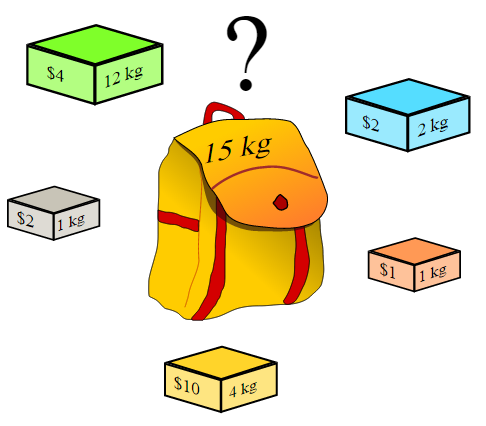
\includegraphics[width=0.5\textwidth]{MarcoTeorico/Imagenes/imagen_mochila.png}
            \caption{Ejemplo del problema de la mochila.}      
            \label{fig:imagen_mochila}
    \end{figure}   
    
Los datos del problema se pueden expresar en términos matemáticos.:
\begin{itemize}
\item Los objetos están numerados por el índice $i$ variando de $1$ a $N$ objetos (ítem).
\item De cada tipo de ítem se tienen $q_i$ ítems disponibles, donde $q_i$ es un entero positivo que cumple $1\leq q_i\leq\infty$.
\item Los números $w_{i}$ y $v_{i}$ representan el peso y el valor del número $i$. 
\item La capacidad de la mochila se denomina en esta fórmula $W$.
\item La solución al problema vendrá dado por la secuencia de variables $x_{n}$ donde el valor de $x_{i}$ indica cuantas copias se meterán en la mochila del tipo de ítem ${i}$
\end{itemize}
Con todo esto se puede formular matemáticamente de la siguiente forma:
%\begin{itemize}
%\item Maximizar $  \Sigma_{i=1}^{n}  v_{i} x_{i}$
%\item De tal manera que  $ \Sigma_{i=1}^{n}  w_{i} x_{i} \leq W $
%\item y $1\leq q_i\leq\infty$
%\end{itemize}

\begin{equation*}
\begin{aligned}
\text{maximizar } & \sum_{i=1}^N v_{i} x_{i} \\
\text{sujeto a }  & \sum_{i=1}^{n}  w_{i} x_{i} \leq W \\
                  & 1\leq q_i\leq\infty.
\end{aligned}
\end{equation*}